\documentclass[../../main]{subfiles}

\input{section_header.tex}

\begin{document}

\section{Main Board} \label{sec:}

The relay board from the previous section will be used for controlling relays. We have actuators
like lights, fans, and humidifiers. So we need another set of shift registers to control them. If
we use \emph{74LS95} here, the lack of an extra storage latch will cause the lights to flicker
as we shift through serial data. So we need a shift register with storage latches. We can pick
\emph{74HC595} for this use case. Refer figures \ref{fig:74hc595Dip} and \ref{fig:74hc595PinDiagram}
for more info about the IC. And table \ref{tbl:74hc595RelventPins} goes through the pins of
\emph{74HC595}.

\alertImportant{
    \emph{74HC595} is a CMOS version of the chip. Inorder to drive them from \esp we need some
    kind of level shifters as the logic high voltage of the \esp will be too low for \emph{74HC595}
    to register as logic high. We can simply use some inverters discussed in the previous sections
    for this purpose. Since we are using inverters as buffers, we need to flip the bits from
    the software to actually shift in the right bits we want.
}

\begin{center}
    {\begin{minipage}[c] {0.35\textwidth}
        \centering

        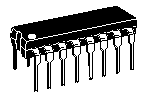
\includegraphics [
        ] {pics/74hc595_dip.pdf}
        \captionof{figure} {
            Dip package of \emph{74HC595}.
            \label{fig:74hc595Dip}
        }

        \includegraphics [
            max width = \IGXMaxWidth,
            max height = \IGXMaxHeight,
            \IGXDefaultOptionalArgs,
        ] {tikzpics/endAbsEightBitShiftRegisterPinout.pdf}
        \captionof{figure} {
            Pin diagram of \emph{74HC595}.
            \label{fig:74hc595PinDiagram}
        }

    \end{minipage}
    \hfill
    \begin{minipage}[c] {0.52\textwidth}

        \centering

        \begin{tabularx} {\linewidth} {
                *{1}{>{\centering\arraybackslash}m{0.27\linewidth}}
                *{1}{>{\centering\arraybackslash}m{0.73\linewidth}}
            }
            \toprule
            Pins & Remarks \\
            \midrule
            \texttt{Q A - Q H} & Parallel output lines. \\
            \texttt{SER} & Serial in. \\
            $\overline{\mbox{\texttt{OE}}}$ & Output Enable (always tied high). \\
            \texttt{RCLK} & Clock pulse for storage latches. \\
            \texttt{SRCLK} & Clock pulse. \\
            $\overline{\mbox{\texttt{SRCLR}}}$ & Clear for shifting latches (always tied high). \\
            \bottomrule
        \end{tabularx}
        \captionof{table} {
            Relevant pins of \emph{74HC595}.
            \label{tbl:74hc595RelventPins}
        }

    \end{minipage}}

\end{center}

\subsection{Building a 24 Bit Shift Register}

The only difference from the previous relay board system is that there will be an
extra clock line for the storage latches from the \esp. Refer figure \ref{fig:absTwentyFourBitShiftRegister}
for the circuit diagram.

\begin{figure}
    \centering
    \includegraphics [
        max width = \IGXMaxWidth,
        max height = \IGXMaxHeight,
        \IGXDefaultOptionalArgs,
    ] {tikzpics/endAbsTwentyFourBitShiftRegister.pdf}
    \captionof{figure} {$3$ \emph{74HC595} ICs are cascaded to form a $24$ bit shift register.}
    \label{fig:absTwentyFourBitShiftRegister}
\end{figure}


\end{document}
